
\bigskip

Sur la figure ci-dessous :

\begin{itemize}[label={\textbullet~}]
	\item BCDE est un rectangle, BAE est un triangle rectangle en A ;
	\item la perpendiculaire à la droite (CD) passant par A coupe cette droite en H;
	\item les droites (AE) et (CD) se coupent en F.
\end{itemize}
\begin{center}
	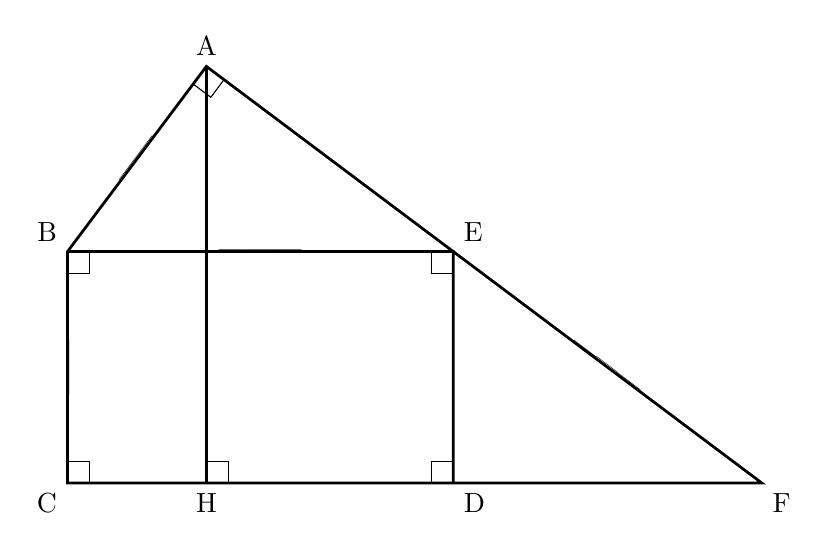
\begin{tikzpicture}[x=7mm,y=7mm]
	\draw[line width=1pt] (0,0) node[below left]{C}--
		(12.6,0.) node[below right] {F}--
		(2.52,7.56) node[pos = 0.28, sloped]{|||} node[above]{A}--
		(0.,4.2)node[pos = 0.5, sloped]{||} node[above left]{B} --cycle node[pos = 0.5, sloped]{||}
		(0.,4.2) -- (7.,4.2)node[pos = 0.5, sloped]{|||} node[above right]{E} -- (7.,0.) node[below right]{D}
		(2.52,0.) node[below] {H} -- (2.52,7.56);
		\foreach \x/\y in {0/0 , 2.52/0, 6.6/0, 6.6/3.8, 0/3.8}
			\draw[shift={(\x,\y)}] (0,0) rectangle (0.4,0.4) ;
		\draw[shift={(2.52,7.56)},rotate=143.13] (0,0) rectangle (-0.4,0.4) ;
\end{tikzpicture}
\end{center}

On donne :
\begin{itemize}[label={\textbullet~}]
	\item $\mathrm{AB}=\mathrm{BC}=4,2 \mathrm{~cm}$;
	\item $\mathrm{EB}=\mathrm{EF}=7 \mathrm{~cm}$.
\end{itemize}

\begin{enumerate}
\item Montrer que l'aire du rectangle BCDE est égale à \np[cm^2]{29,4}.
\item 
	\begin{enumerate}
		\item Montrer que la longueur AE est égale à \np[cm]{5,6}.
		\item Calculer l'aire du triangle rectangle ABE.
	\end{enumerate}
\item 
	\begin{enumerate}
		\item Montrer que les droites (ED) et (HA) sont parallèles.
		\item Calculer la longueur AH.
	\end{enumerate}
\end{enumerate}

\vspace{5mm}

